\documentclass{beamer}
\usetheme{metropolis}

\usetheme{metropolis}

\usepackage[ngerman]{babel}
\usepackage[autostyle=true,german=quotes]{csquotes}
\usepackage[linewidth=1pt]{mdframed}
\usepackage{hyperref}
\usepackage{makecell}
\usepackage{pifont}
\usepackage{tikz}
\usetikzlibrary{positioning, calc, arrows, fit, decorations.pathreplacing, shapes, shapes.multipart, snakes}
\usepackage{verbatim}
\usepackage{textcomp}
\usepackage{centernot}
\usepackage{tabularx}
\usepackage{ulem}
%\usepackage{pdfpages}

\batchmode

\hypersetup{
	colorlinks,
	urlcolor=blue,
	linkcolor=black % for ToC
}
\newenvironment{qaa}[1]{
	#1

	\begin{mdframed}
		\small
}{
	\end{mdframed}
}

\newcommand{\true}{\ding{51}}
\newcommand{\false}{\ding{55}}
\newcommand{\code}[1]{
	\begin{mdframed}
		\verbatiminput{#1}
	\end{mdframed}
}


\title{Tutorium 03: Typen und Typklassen}
% \subtitle{}
\author{Paul Brinkmeier}
\institute{Tutorium Programmierparadigmen am KIT}
\date{09. November 2020}

\begin{document}

\begin{frame}
	\titlepage
\end{frame}

\section{Übungsblatt 2}

\begin{frame}{2.1 -- Bindung und Gültigkeitsbereiche}
    \begin{figure}
        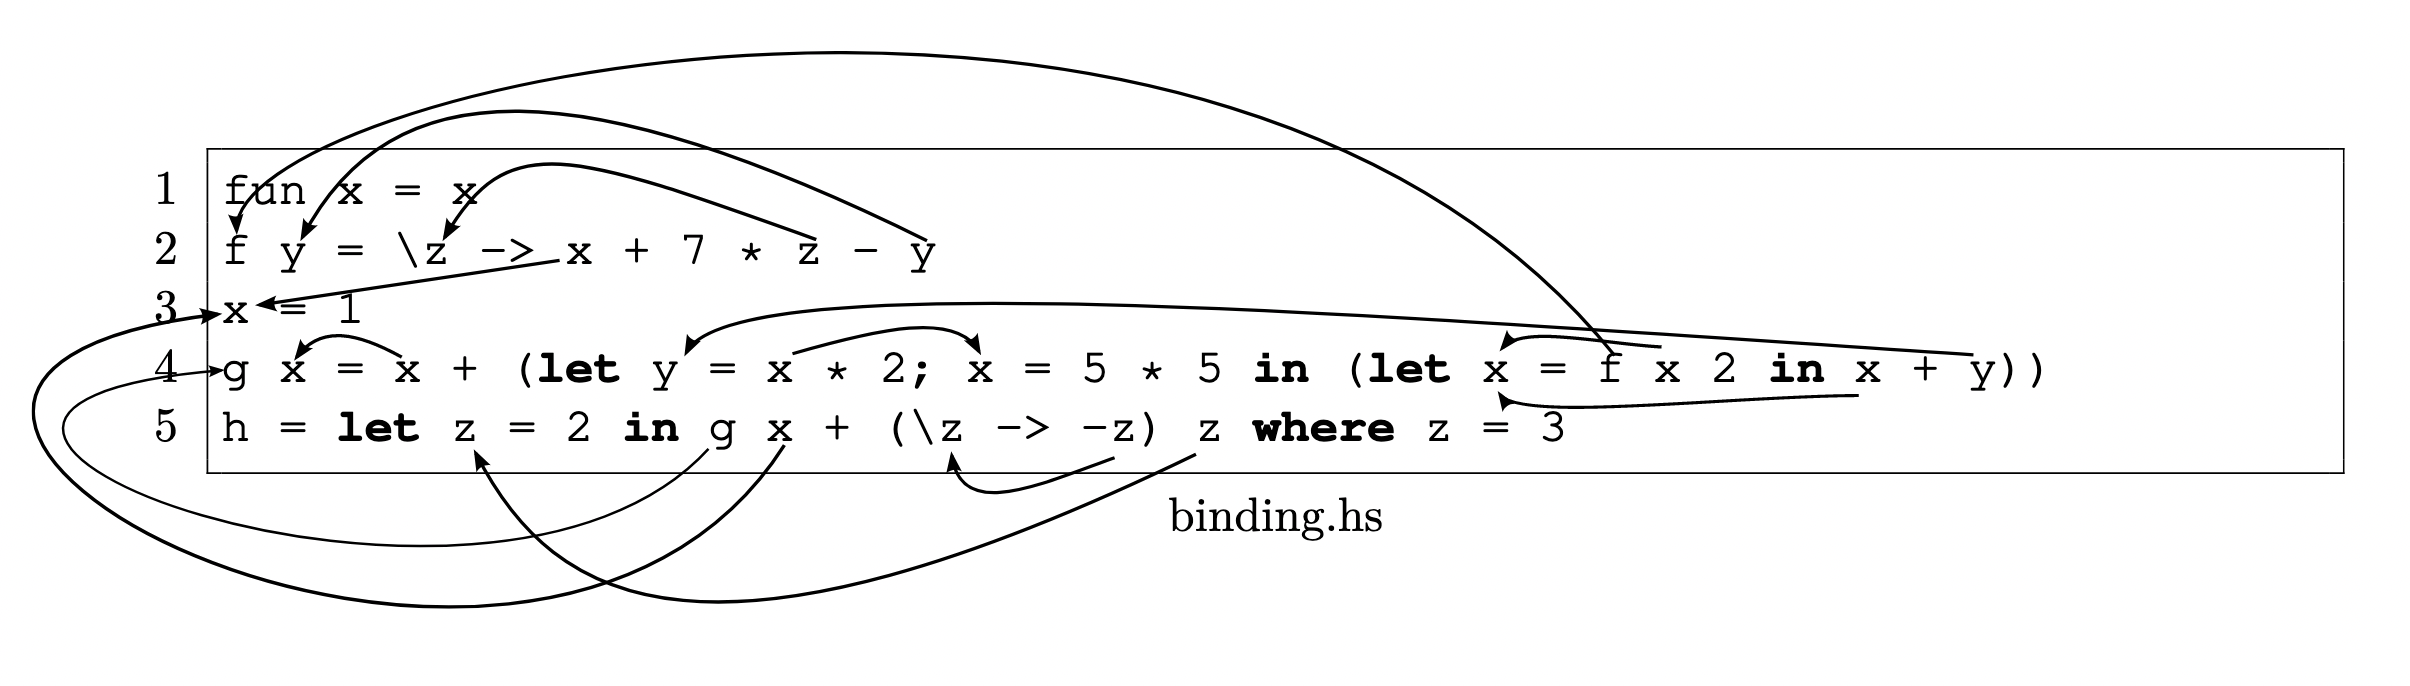
\includegraphics[width=\textwidth]{images/binding.png}
    \end{figure}

    \begin{itemize}
        \item Größte Fehlerquelle: \texttt{x * 2} und \texttt{f x 2} in Zeile 4
        \item Beide zeigen auf Definition im selben \texttt{let}-Block
        \item $\leadsto$ Allgemein: Variablen zeigen möglicherweise auf eine Definition im selben \texttt{let}-Block, selbst wenn es ihre eigene ist.
    \end{itemize}
\end{frame}

\begin{frame}{2.2.\{1,2,3\} -- Polynome}
  \code{../demos/Polynom.hs}

  \texttt{(\$) :: (a -> b) -> a -> b} -- Funktionsanwendung als Operator.
\end{frame}

\section{Wiederholung:\\Typen und Typklassen}

\begin{frame}{Cheatsheet: Typen}
  \begin{itemize}
    \item \texttt{Char}, \texttt{Int}, \texttt{Integer}, ...
    \item \texttt{String}
    \item \emph{Typvariablen}/\emph{Polymorphe Typen}:
    \begin{itemize}
      \item \texttt{(a, b)}: Tupel
      \item \texttt{[a]}: Listen
      \item \texttt{a -> b}: Funktionen
      \item Vgl. Java: \texttt{List<A>}, \texttt{Function<A, B>}
    \end{itemize}
    \item \emph{Typsynonyme}: \texttt{type String = [Char]}
  \end{itemize}
\end{frame}

\begin{frame}{Cheatsheet: Algebraische Datentypen in Haskell}
  \begin{itemize}
    \item \emph{\texttt{data}-Definitionen}, \emph{Datenkonstruktoren}
    \item Algebraische Datentypen: \emph{Produkttypen} und \emph{Summentypen}
    \begin{itemize}
      \item Produkttypen $\approx$ \texttt{struct}s in C
      \item Summentypen $\approx$ \texttt{enum}s
    \end{itemize}
    \item \emph{Typkonstruktoren}, bspw. \texttt{[] :: * -> *}
    \item \emph{Polymorphe} Datentypen, bspw. \texttt{[a]}, \texttt{Maybe a}
    \item Beispiel:
  \end{itemize}
  \code{../demos/Shape.hs}
\end{frame}

\begin{frame}{Cheatsheet: Typklassen 1}
  \begin{itemize}
    \item \emph{Klasse}, \emph{Operationen}/\emph{Methoden}, \emph{Instanzen}
    \item Beispiele:
    \begin{itemize}
      \item \texttt{Eq t}, $\{ \texttt{(==)}, \texttt{(/=)} \}$, $\{ \texttt{Eq Bool}, \texttt{Eq Int}, \texttt{Eq Char}, ... \}$
      \item \texttt{Show t}, $\{ \texttt{show} \}$, $\{ \texttt{Show Bool}, \texttt{Show Int}, \texttt{Show Char}, ... \}$
    \end{itemize}
    \item Weitere Typklassen: \texttt{Ord}, \texttt{Num}, \texttt{Enum}
    \item Deklaration/Implementierung:
  \end{itemize}

  \code{../demos/Truthy.hs}
\end{frame}

\begin{frame}{Cheatsheet: Typklassen 2}
  \begin{itemize}
    \item \emph{Vererbung}: Typklassen mit Voraussetzungen
  \end{itemize}

  \code{../demos/Truthy2.hs}
\end{frame}

\begin{frame}{\texttt{type}: Namen für Typen}
    \begin{alignat*}{2}
        & \texttt{type} \quad \texttt{String} \quad && \texttt{=} \quad \texttt{[Char]} \\
        & \texttt{type} \quad \texttt{Rational} \quad && \texttt{=} \quad \texttt{Ratio Integer} \\
        & \texttt{type} \quad \texttt{FilePath} \quad && \texttt{=} \quad \texttt{String} \\
        & \texttt{type} \quad \texttt{IOError} \quad && \texttt{=} \quad \texttt{IOException}
    \end{alignat*}

    \begin{itemize}
        \item \texttt{type N = T} definiert einen neuen Typnamen \texttt{N} für den Typen \texttt{T}
        \item \texttt{N} kann nun überall verwendet werden wo auch \texttt{T} es kann
        \item $\leadsto$ Bessere Lesbarkeit\\
              (bspw. \texttt{readFile :: FilePath -> IO String})
    \end{itemize}
\end{frame}

\begin{frame}{\texttt{data}: Neue Typen}
    \texttt{data} definiert einen neuen Typen $t$ durch die Aufzählung aller seiner \enquote{Konstruktoren} $c_i$:

    \begin{alignat*}{2}
        & \texttt{data} \quad \texttt{Bool} \quad && \texttt{=} \quad \texttt{False} \\
        &               \quad               \quad && \texttt{|} \quad \texttt{True}  \\
        \\
        & \texttt{data} \quad t             \quad && \texttt{=} \quad c_1            \\
        &               \quad               \quad && \texttt{|} \quad c_2            \\
        &               \quad               \quad && \texttt{|} \quad ...            \\
        &               \quad               \quad && \texttt{|} \quad c_n            \\
    \end{alignat*}

    Jeder Konstruktur $c_i$ hat einen Namen und ggf. Parameter.
\end{frame}

\begin{frame}{\texttt{data}: Beispiel komplexe Zahlen}
    \code{../demos/Complex.hs}

    \begin{itemize}
        \item Zwei Darstellungen: $z = a + b\text{i} = r * (\cos \phi + \text{i} \sin \phi)$
        \item Beide Darstellungen bestehen aus zwei reellen Zahlen
        \item $\leadsto$ Durch unterschiedliche Konstruktornamen unterscheiden
    \end{itemize}
\end{frame}

\begin{frame}{\texttt{data}: Beispiel Bruchzahlen}
    \begin{itemize}
        \item Bruch ist ein Tupel von Integern
        \item Wie würde die Multiplikation aussehen
    \end{itemize}
    \pause
    \code{../demos/Fraction.hs}

    \begin{itemize}
        \item Definition von \texttt{Fraction} gibt uns Typsicherheit:\\
              Ein Bruch bleibt ein Bruch
        \item Konvention: Hat ein Typ nur einen Konstruktor, benennen wir diesen nach dem Typen.
    \end{itemize}
\end{frame}

\section{Übung}

\begin{frame}{Queues}
  Warteschlangen lassen sich in Haskell, nicht effizient als Liste implementieren, weil die enqueue Operation immer die gesamte Liste durchlaufen muss. Folgende Definition schafft abhilfe
  
  \texttt{data Queue a = Q [a] [a]}

  \texttt{Q front back} stellt die Queue dar, die durch Konkatenation von \texttt{front} und der Umkehrung von \texttt{back} entsteht

  Implementieren sie \texttt{fromList::[a] -> Queue a} und \texttt{toList::Queue a -> [a]}
\end{frame}

\begin{frame}{Queues}
    Implementieren sie folgende Funktionen:
    \begin{itemize}
        \item \texttt{enqueue::a -> Queue a} mit konstanter Anzahl Speicherzugriffe
        \item \texttt{dequeue::Queue a -> Maybe (a, Queue a)}
    \end{itemize}
\end{frame}

\begin{frame}{Queues}
    Instanziieren sie die Typklasse \texttt{Eq} für den Datentyp \texttt{Queue}
\end{frame}

\begin{frame}{Führerschein}
  \code{../demos/DriversLicense.hs}

  \vfill

  \begin{itemize}
    \item Klasse B kann Zusatzziffer B96 haben.
    \item Für Daten gibt es natürlich auch eigene Typen.
    \item Beispiel:\\
          \texttt{DriversLicense [A, B True] "{}Arthur"{} (1, 1, 1970)}
  \end{itemize}
\end{frame}

\begin{frame}{Spielkarten}
  \code{../demos/PlayingCard.hs}
\end{frame}

\begin{frame}{Monopolykarten}
  \code{../demos/Monopoly.hs}
\end{frame}

\begin{frame}{Boolesche Logik}
  \code{../demos/BoolExpr.hs}

  \vfill

  Beispiele:
  \begin{itemize}
    \item $a \wedge b$ entspricht \texttt{BinaryOp (Var "{}a"{}) AND (Var "{}b"{})}
    \item $a \vee (b \wedge 0)$ entspricht\\
          \texttt{BinaryOp (Var "{}a"{}) AND (BinaryOp (Var "{}b"{}) OR (Const False))}
  \end{itemize}
\end{frame}

\begin{frame}{MiMa}
  \code{../demos/MiMa.hs}
\end{frame}

\section{Typklassen implementieren}

\begin{frame}{Implementierung von Typklassen}
  Implementiert:

  \vfill

  \begin{itemize}
    \item Monopolykarten: \texttt{Eq MonopolyCard}, \texttt{Show MonopolyCard}
    \item Boolesche Ausdrücke: \texttt{Show BoolExpr}
    \item Typen in Haskell: \texttt{Show Type}
    \item MiMa-Instruktionen: \texttt{Show MiMaInst}
    \item Spielkarten: \texttt{Eq} und \texttt{Ord} für \texttt{Suit}, \texttt{Rank} und \texttt{PlayingCard}
    \begin{itemize}
      \item \texttt{Ord PlayingCard}: Zuerst nach Farbe, dann nach Wert.
    \end{itemize}
  \end{itemize}

  \vfill
  
  Aufgabe: Spielkarten + eine weitere
\end{frame}

\begin{frame}{\texttt{Ord PlayingCard} -- Vorlage}
  \code{../demos/PlayingCard2.hs}
\end{frame}

\begin{frame}{\texttt{Ord PlayingCard} -- Automatische Instanz durch \texttt{deriving}}
  \code{../demos/PlayingCard3.hs}

  \texttt{Enum} ermöglicht es, bspw. \texttt{[Hearts .. Spades]} zu schreiben.
\end{frame}

\end{document}
